% !TeX program = lualatex
% Agregátor reálných otázek SZZ pro okruh S1. Jednotlivé otázky jsou v souborech q_*.tex.
% Sestavení: ./build.sh 03_specializace_ui_su/S1_zaklady_ui/priklady   (nebo cd .../priklady && latexmk)
\documentclass[11pt,a4paper]{article}
\usepackage{szzpriklady}
% Build běží z adresáře priklady/ (CWD), obrázky jsou v src/fig/.
\graphicspath{{src/fig/}{fig/}}

\title{Příklady otázek -- Základy umělé inteligence\\[0.3em]\large Reálné otázky ze SZZ 2022--2026 (S1)}
\author{Jakub Klesa}
\date{Pokryté předměty: NAIL120 (Úvod do umělé inteligence)}

\begin{document}
\sloppy
\maketitle
\tableofcontents
\bigskip

\begin{poznamka}
Tento dokument obsahuje reálné otázky z minulých termínů SZZ (2022--2026) zařazené do
okruhu S1. U otázek s obrázkem je grafika oříznutá z originálního PDF (viz odkaz na
zdroj). Text, číselná data a tabulky jsou přepsané věrně.
Zadání i oficiální náčrty řešení pocházejí ze sad zveřejněných na webu MFF UK:\par
{\raggedright\url{https://www.mff.cuni.cz/cs/studenti/bakalarske-studium/statni-zaverecne-zkousky/bakalarske-statni-zkousky-studijniho-programu-informatika}\par}
Náčrty označené jako doplněné jsou vlastní, oficiální sada je k~dané otázce neobsahuje.
Vlastní doplnění k~oficiálnímu náčrtu jsou zřetelně oddělena.
Pojmy a~značení odpovídají přednáškám předmětu NAIL120 \emph{Úvod do umělé inteligence}
(R.~Barták, \url{https://ktiml.mff.cuni.cz/~bartak/ui_intro/}) a~učebnici S.~Russella
a~P.~Norviga \emph{Artificial Intelligence: A~Modern Approach} (\url{https://aima.cs.berkeley.edu/}).
\end{poznamka}
\bigskip

% === Otázky (chronologicky). Doplň \input řádky a soubory q_*.tex do src/. ===
% Příklad: % Zdroj: PDF priklady-leto-2024.pdf, fyzická str. 23. Značka: specializace UI-SU, UI-ZPJ. Zařazeno: S1 (bayesovské sítě). CPT tabulky jsou součástí obrázku.
\section{Bayesovské sítě}
\szzotazka{léto 2024}{28}{Bayesovské sítě}

\noindent\textbf{Zadání.}\par
Definujte Bayesovskou síť a napište, jak se takové sítě používají a jak se konstruují. Jaký je vztah mezi Bayesovskou sítí a úplnou sdruženou pravděpodobnostní distribucí?

Uvažujte níže zobrazenou Bayesovskou síť se 4 náhodnými proměnnými $P_1, \dots, P_4$ a uvedenými podmíněnými pravděpodobnostními distribucemi. Máme pozorování $P_3 = F$ a $P_4 = T$. Spočítejte, jaká je pravděpodobnost, že $P_1 = T$, tedy $P(P_1 = T \mid P_3 = F, P_4 = T)$.

\begin{center}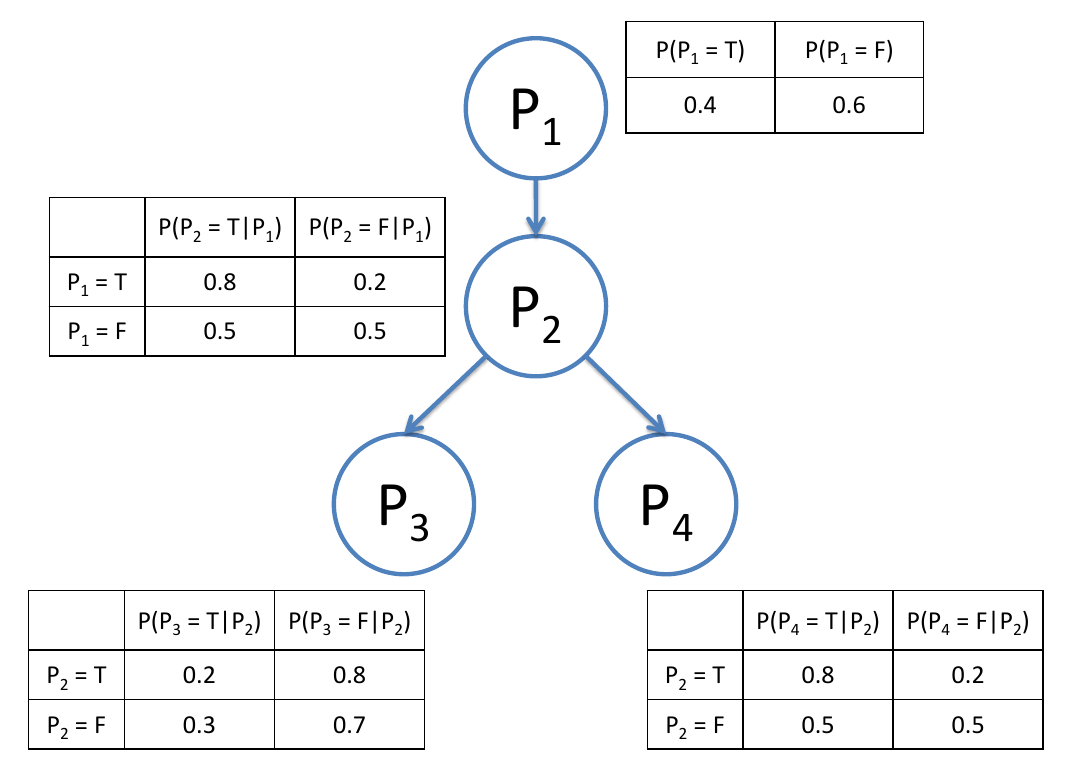
\includegraphics[width=0.85\linewidth]{bayesovske-site.png}\end{center}

\medskip
\noindent\textbf{Řešení.} \textit{(V~PDF bez náčrtu řešení; vlastní vzorové řešení, výpočet ověřen numericky.)}\par

\noindent\emph{Definice a vztah ke sdružené distribuci.} Bayesovská síť je orientovaný acyklický graf, jehož uzly jsou náhodné veličiny, hrana $X\to Y$ značí přímý vliv (rodičovství) a~každý uzel nese tabulku podmíněných pravděpodobností (CPT) $P(X\mid \mathrm{Parents}(X))$. Síť \emph{plně reprezentuje} úplnou sdruženou distribuci součinem CPT:
\[ P(x_1,\dots,x_n)=\prod_i P\big(x_i\mid \mathrm{Parents}(X_i)\big). \]
Používá se k~odpovídání na dotazy $P(X\mid \text{evidence})$; konstruuje se seřazením veličin (ideálně příčiny před důsledky) a~výběrem minimální množiny rodičů pro každou veličinu.

\noindent\emph{Výpočet} $P(P_1{=}T\mid P_3{=}F,P_4{=}T)$. Síť je řetěz $P_1\to P_2\to\{P_3,P_4\}$ ($P_2$ je rodič $P_3$ i~$P_4$). Vysčítáme skrytou $P_2$:
\begin{align*}
P(P_1{=}T,P_3{=}F,P_4{=}T) &= P(P_1{=}T)\sum_{P_2} P(P_2\mid P_1{=}T)\,P(P_3{=}F\mid P_2)\,P(P_4{=}T\mid P_2)\\
&= 0{,}4\,[\,0{,}8\cdot0{,}8\cdot0{,}8 + 0{,}2\cdot0{,}7\cdot0{,}5\,]=0{,}4\cdot0{,}582=0{,}23280,\\
P(P_1{=}F,P_3{=}F,P_4{=}T) &= 0{,}6\,[\,0{,}5\cdot0{,}8\cdot0{,}8 + 0{,}5\cdot0{,}7\cdot0{,}5\,]=0{,}6\cdot0{,}495=0{,}29700.
\end{align*}
Normalizace ($P(P_3{=}F,P_4{=}T)=0{,}23280+0{,}29700=0{,}52980$):
\[ P(P_1{=}T\mid P_3{=}F,P_4{=}T)=\frac{0{,}23280}{0{,}52980}=\boxed{0{,}4394}\quad(\approx 43{,}9\,\%). \]
(Použito $P(P_3{=}F\mid P_2{=}T)=1-0{,}2=0{,}8$ a~$P(P_3{=}F\mid P_2{=}F)=1-0{,}3=0{,}7$.) Pozorování $P_3,P_4$ tak zvedlo víru v~$P_1{=}T$ z~apriorních $0{,}4$ na~$0{,}439$.

% ZACATEK-OTAZEK
\input{src/q_2022-leto-09_n-kralovny}
\input{src/q_2022-podzim-17_barveni-grafu-dpll}
\input{src/q_2023-jaro-05_planovani}
\input{src/q_2023-leto-05_hmm}
\input{src/q_2023-podzim-28_csp}
\input{src/q_2024-jaro-32_informovane-prohledavani}
\input{src/q_2024-leto-28_bayesovske-site}
\input{src/q_2024-podzim-28_minimax}
\input{src/q_2025-jaro-27_dpll-parovani}
\input{src/q_2025-jaro-30_bayesovske-uceni}
\input{src/q_2025-leto-29_bellmanova-rovnice}
\input{src/q_2025-podzim-27_jednotahove-hry}
\input{src/q_2026-jaro-27_csp}
% KONEC-OTAZEK

\end{document}
